\documentclass{article}

\usepackage{amsmath}
\usepackage{bm}
\usepackage{caption}
\usepackage{genealogytree}
\usepackage{hyperref}
\usepackage{listings}
\usepackage{struktex}
\usepackage{tabularx}
\usepackage{tikz}
\usetikzlibrary{positioning}
\usetikzlibrary{shapes}
\usetikzlibrary{shapes.geometric}
\tikzset{
  box/.style={rectangle, draw},
}

\usepackage{xcolor}
\definecolor{light-gray}{gray}{.9}

\author{Karsten Lehmann}
\date{WiSe 2020}
\title{Mitschriften Programmieren - Grundlegende Konzepte (PR10)}

\begin{document}

\maketitle

\vfill
\begin{center}
  Dozent: Prof. Dr. Wolfgang V. Walter \\
  \href{mailto:wolfgang.walter@tu-dresden.de}{wolfgang.walter@tu-dresden.de}
\end{center}

\newpage

\section{Einführung}

\fcolorbox{black}{light-gray}{\begin{minipage}{\textwidth}
    David Hilbert \gtrsymBorn~23. Januar 1862 \gtrsymDied~14. Februar 1943 \\

    Bedeutender Deutscher Mathematiker mit vielen Beiträgen zu einzelnen Bereichen der Mathematik und
    Vertreter des Formalismus der Mathematik.
\end{minipage}}

\noindent
\textbf{Programmiersprache} ist eine Sprache, die lexikalisch, syntaktisch und semantisch eindeutig definiert ist.
Texte sind vom Menschen les- und schreib-bar, sowie vom Computer eindeutig interpretierbar.

\noindent
\textbf{Compiler} übersetzt den Programmtext in Maschinensprache

\noindent
\textbf{Interpreter} arbeitet ein Programm direkt ab

\noindent
\textbf{Laufzeitsystem} stellt grundlegende Funktionen zur Ausführung und Abarbeitung eines Programms zur Verfügung.

\begin{tikzpicture}
  \node[box] (prob) {Problem ???};
  \node[align=left, below left = 0cm and 1cm of prob] (analysis) {Analyse\\ des Problems};
  \node[below = of prob, box] (algo) {
    Algorithmus
    \begin{struktogramm}(40,20)
      \assign{bestimme Startwert}
      \until{wiederhole, bis genau genug}
      \assign{Iteration}
      \untilend
    \end{struktogramm}
  };
  \node[align=left, below left = 0cm and -2.5cm of algo] (code) {Kodierung in einer \\Programmiersprache};
  \node[below = 5em of algo, box] (prog) {
    Programm
    \begin{lstlisting}[frame=single,language=Pascal, linewidth=16em]
x := 1.5;
repeat
  xalt := x;
  x := x - f(x) / f^(x)
until (abs (x-xalt) < eps);
\end{lstlisting}
  };
  \node[rectangle, draw, rounded corners = .1cm, above right = .5cm and -.5cm of prog] (input) {Eingabe};
  \node[rectangle, draw, rounded corners = .1cm, below right = .5cm and -.5cm of prog] (output) {Ausgabe};

  
  \node[diamond, draw, below = of prog] (ok) {Okay?};
  \node[align=left, left = of ok] (exec_test) {Ausführung \\und Test};
  \node[box, below = of ok] (lsg) {Lösung};

  \node[below left = .5cm and 0cm of ok] {alles richtig};
  \node[below right = 0cm and .5cm of ok] {Fehler gefunden};
  
  \node[align=left, box, right = .3cm of prog] (e_prog) {Fehler im \\Programm};
  \node[align=left, box, above right = .5cm and -.4cm of e_prog] (e_algo) {Fehler im \\Algorithmus};
  \node[align=left, box, above right = .5cm and -.8cm of e_algo] (e_prob) {Problem \\überdenken};
  
  \draw[-latex] (prob.south) -> (algo.north);
  \draw[-latex] (algo.south) -> (prog.north);
  \draw[-latex] (prog.south) -> (ok.north);
  \draw[-latex] (ok.south) -> (lsg.north);
  
  \draw[-latex] (ok.east) -| (e_prog.south);
  \draw[-latex] (ok.east) -| (e_algo.south);
  \draw[-latex] (ok.east) -| (e_prob.south);
  \draw[-latex] (e_prob.north) |- (prob.east);
  \draw[-latex] (e_algo.north) |- ([xshift=6.5em]analysis.east);
  \draw[-latex] (e_prog.north) |- ([xshift=3em]code.east);

  \draw[-latex] (input.south) -> ([xshift=3cm]prog.north);
  \draw[-latex] ([xshift=3cm]prog.south) -> (output.north);
\end{tikzpicture}

\subsection{Algorithmen}

Ein Algorithmus ist ein endliches und vollständiges System von in einer formalen, eindeutig interpretierbaren
Sprache oder Notation geschriebenen Regeln zur schrittweisen Lösung einer Klasse von Problemen in endlicher
Zeit.

\subsection*{Die 3 Grundstrukturen eines Algorithmus}

\subsubsection*{Sequenz}

Eine Sequenz ist eine Folge von Aktionen / Schritten / Befehlen / Anweisungen, welche in der Reihenfolge ihres Auftretens im Programm
abgearbeitet werden.
Innerhalb der anderen Grundstrukturen bezeichnet man die Sequenz als \emph{Anweisungsblock}.

\subsubsection*{Selektion}

Eine Selektion (Auswahl / Verzweigung) wählt anhand einer Entscheidung aus, welche an welcher Stelle der Algorithmus fortgesetzt wird.
Der Standardfall ist das if-then-else Konstrukt, in dem auf Basis einer binären Entscheidung gewählt wird, welcher
Anweisungslock ausgeführt wird.
Viele Sprachen bieten auch die Möglichkeit einer Mehrfachverzweigung.

\subsubsection*{Repetition}

Eine Repetition (Wiederholung / Zyklus / Schleife) erlaubt die Mehrfache Abarbeitung eines Anweisungsblockes im Inneren der Schleife.
Manche Sprachen erlauben auch das Verlassen der Schleife aus dem Schleifenkörper mittel \emph{break} oder \emph{exit}.

\subsection*{Unterporgramme, Prozeduren, Funktionen}

Die Prozedur ist die 4. Strukturierungsmöglichkeit für Programmcode. Mit dieser kann man logisch zusammengehörige Teile eines Algorithmus
gruppieren.

Prozeduren sind in der Regel parametrisiert. Ein Teilalgorithmus, der ein Ergebnis liefern soll wird \textbf{Funktion} genannt, wobei Teilalgorithmen
unabhängig davon, ob Sie Ergebnisse liefern oder nicht in neueren Sprachen als Funktionen bezeichnet werden.

\subsection*{Flussdiagramme}

\begin{tabularx}{\textwidth}{X X}
  Anfang / Ende &
  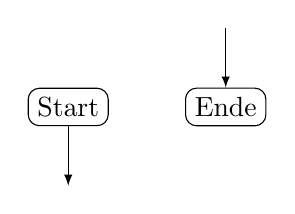
\begin{tikzpicture}[baseline]
    \node[draw, rectangle, rounded corners] at (0,0) (start) {Start};
    \node[draw, rectangle, rounded corners] at (2,0) (end) {Ende};

    \draw[-latex] (2,1) -> (end.north);
    \draw[-latex] (start.south) -> (0,-1);
  \end{tikzpicture}
  \\
  Ein- / Ausgabe &
  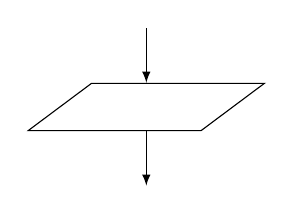
\begin{tikzpicture}[baseline]
    \node[draw, minimum height = .6cm, minimum width = 3cm, trapezium, trapezium left angle=60, trapezium right angle=-60, trapezium stretches = true] at (0,0) (input) {};
    \draw[-latex] (0,1) -> (input.north);
    \draw[-latex] (input.south) -> (0,-1);
  \end{tikzpicture}
  \\
  Anweisung (Aktion) &
  \begin{tikzpicture}[baseline]
    \node[draw, rectangle, minimum height = .6cm,  minimum width = 3cm] at (0,0) (action) {}; 
    \draw[-latex] (0,1) -> (action.north);
    \draw[-latex] (action.south) -> (0,-1);
  \end{tikzpicture}
  \\
  Verzweigung &
  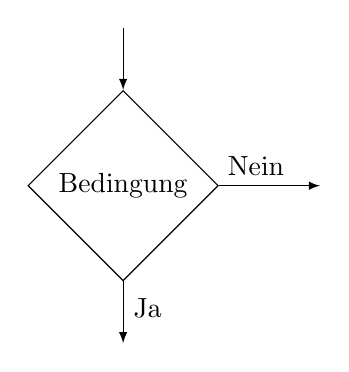
\begin{tikzpicture}[baseline]
    \node[draw, diamond] at (0,0) (selection) {Bedingung};
    \node[below right = .7cm and -.6cm of selection] {Ja};
    \node[above right = -.6cm and .6cm of selection] {Nein};
    \draw[-latex] (0,2) -> (selection.north);
    \draw[-latex] (selection.south) -> (0,-2);
    \draw[-latex] (selection.east) -> (2.5,0);
  \end{tikzpicture}
  \\
  Ablauf / Zusammenführung &
  \begin{tikzpicture}[baseline]
    \draw[-latex] (0,0) -> (1.5,0);
    \draw[-latex] (2,.75) -> (2,-.75);
    \draw[-latex] (3.5,0) -> (2,0);
  \end{tikzpicture}
  \\
  Anschlußstelle zwischen zwei Programmablaufteilen &
  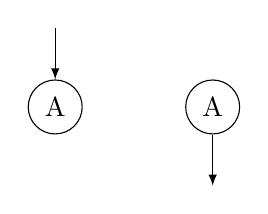
\begin{tikzpicture}[baseline]
    \node[circle, draw] at (0,0) (left) {A};
    \node[circle, draw] at (2,0) (right) {A};
    \draw[-latex] (0,1) -> (left.north);
    \draw[-latex] (right.south) -> (2,-1);
  \end{tikzpicture}
  \\
  Aufruf von Teilalgorithmen &
  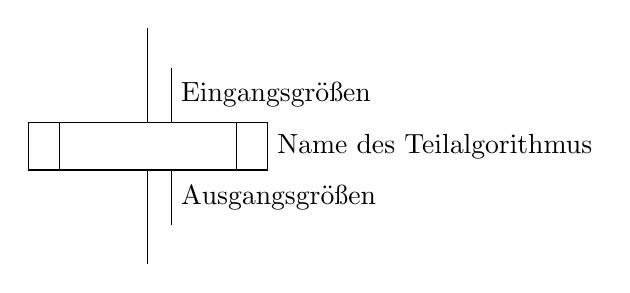
\begin{tikzpicture}[baseline]
    \node[draw,label=right:Name des Teilalgorithmus, rectangle split, rectangle split horizontal, rectangle split parts = 3, minimum height = .6cm] at (0,0) (call) {\nodepart{two}\hspace*{2cm}};
    \draw (0,1.5) -- (call.north);
    \draw (0.3,1) -- node[right] {Eingangsgrößen} ([xshift=.3cm]call.north);
    \draw (call.south) -- (0,-1.5);
    \draw ([xshift=.3cm]call.south) -- node[right] {Ausgangsgrößen} (0.3,-1);
  \end{tikzpicture}
  \\
\end{tabularx}

\subsection*{Struktogramme / Nassi-Shneidermann-Diagramme}

\begin{tabularx}{\textwidth}{l X}
  Anweisung &
  \begin{struktogramm}(40,10)
    \assign{Anw}
  \end{struktogramm}
  \\
  Sequenz &
  \begin{struktogramm}(40,20)
    \assign{Anw\_1}
    \assign{Anw\_2}
    \assign{$\dots$}
    \assign{Anw\_n}
  \end{struktogramm}
  \\
  Selektion &
  \begin{tabular}{c c}
    \begin{struktogramm}(50,20)
      \ifthenelse{2}{2}{Bedingung}{Ja}{Nein}
        \assign{Anw}
      \change
        \assign{}
      \ifend
    \end{struktogramm}
    &
    \begin{struktogramm}(50,20)
      \ifthenelse{2}{2}{Bedingung}{Ja}{Nein}
        \assign{Anw\_1}
      \change
        \assign{Anw\_2}
      \ifend
    \end{struktogramm}
    \\
    einseitige & zweiseitige \\
    \begin{struktogramm}(50,20)
      \case[10]{0}{4}{Fallausdruck}{Wert\_1}
        \assign{Anw\_1}
      \switch{Wert\_2}
        \assign{Anw\_2}
      \switch{$\dots$}
        \assign{$\ldots$}
      \switch{}
        \assign{Anw\_n}
      \caseend
    \end{struktogramm}
    &
    \begin{struktogramm}(60,20)
      \case[10]{3}{5}{Fallausdruck}{Wert\_1}
        \assign{Anw\_1}
      \switch{Wert\_2}
        \assign{Anw\_2}
      \switch{$\dots$}
        \assign{$\ldots$}
      \switch{}
        \assign{Anw\_n}
      \switch[r]{sonst}
        \assign{Anw\_0}
      \caseend
    \end{struktogramm}
    \\
    Mehrfachauswahl ohne und & mit Sonst-Zweig \\

  \end{tabular}
  \\
  Zyklus &
  \begin{tabular}{c c}
    \begin{struktogramm}(60,10)
      \while{Wiederhole solange Bed wahr ist}
        \assign{Anw}
      \whileend
    \end{struktogramm}
    &
    \begin{struktogramm}(60,10)
      \until{Wiederhole bis Bed wahr ist}
        \assign{Anw}
      \untilend
    \end{struktogramm}
    \\
    abweisender & nicht-abweisender \\
    \begin{struktogramm}(60,10)
      \while{Lv := awert (s) ewert}
        \assign{Anw}
      \whileend
    \end{struktogramm}
    \\
    Zählzyklus \\
  \end{tabular}
  \\
\end{tabularx}

\section{Maß- und Speichereinheiten, Größenordnungen}

\subsection{Grundeinheiten}

\fcolorbox{black}{light-gray}{\begin{minipage}{\textwidth}
    Hexadezimalzahlen \\

    Hexadezimalzahlen sind Zahlen, welche zur Basis 16 dargestellt werden. Dabei ist Hexadezimal ein Mischwort aus
    dem griechischen \emph{hexa} für Sechs und dem lateinischen \emph{decem} für 10.
    Korrekte Namen wären Sedezimalzahlen von lateinisch \emph{sedecim} (Sechzehn) oder Hexadekadische Zahlen (griechisch).
\end{minipage}} \\

\textbf{Zahlkonversion}: binär $\Leftarrow$ dezimal

\begin{align*}
  10 &= [1010]_2 \\
  57 &= [111001]_2 \\
\end{align*}

\[
  \begin{array}{ cccc cccc }
     &1&1&1&0&0&1 &: 10101 = 101_2 \text{ Rest } 111_2 = 5_{10} \text{ Rest } 7_{10} \\
    -&1&0&1&0) \\
    \cline{1-4}
     &0&1&0&0&0 \\
    -& &0&0&0&0 \\
    \cline{2-6}
     &0&1&0&0&0&1 \\    
    -& & &1&0&1&0 \\
    \cline{3-7}
     & &0&0&1&1&1 \\    
  \end{array}
\]

\[
  \Rightarrow 111001_2 = 57_{10}
\]

\textbf{Zweierkomplement-Addition}:

\begin{minipage}[t]{.4\textwidth}
  \[
    \begin{array}{ccc}
       & 0101_2 &= 5_{10} \\
      +& 1000_2 &= -8_{10} \\
      \cline{1-2}
       & 1101_2 &= -3_{10} \\
    \end{array}
  \]
\end{minipage}
\hfill
\vrule
\hfill
\begin{minipage}[t]{.4\textwidth}
  \[
    \begin{array}{ccc}
       & 0101_2 &= 5_{10} \\
      +& 0101_2 &= 5_{10} \\
      \cline{1-2}
       & 1010_2 &= -6_{10} = 10_{10} - 16_{10}\\
    \end{array}
  \]
\end{minipage}  \\

\begin{minipage}[t]{.4\textwidth}
  \[
    \begin{array}{ccc}
       & 1011_2 &= -5_{10} \\
      +& 1011_2 &= -5_{10} \\
      \cline{1-2}
       & 1110_2 &= 6_{10} = -10_{10} + 16_{10} \\
    \end{array}
  \]
\end{minipage}  \\

\textbf{Zweierkomplement-Subtraktion}:

\[
  a - b = a + (-b) = a + \bar{b} + 1
\]

\[
  \begin{array}{ccc}
      & a \\
    + & \bar{b} \hspace{5pt} &\text{(1er Komplement)} \\
    + & 1                    &\text{(hinterer Übertrag)}\\
    \cline{1-3}
      & a - b \\
  \end{array}
\]

\textbf{Gebrochenen Anteil konvertieren}:

\begin{minipage}[t]{.4\textwidth}
  \[
    \begin{array}{cccc cccc cc}
      0.&1&1&0&1 &* &1&0&1&0 \\
      \cline{0-9}
        & & & &  &  &0&0&0&0 \\
        & & & &  &1 &1&0&1 \\
        & & & &0 &0 &0&0 \\
        & & &1&1 &0 &1 \\
      \cline{0-9}
      \bm{8}&=&\bm{1}&\bm{0}&\bm{0}&\bm{0}.&0&0&1&0 \\
    \end{array}
  \]
\end{minipage}
\hfill
\vrule
\hfill
\begin{minipage}[t]{.4\textwidth}
  \[
    \begin{array}{cccc cccc cc}
      0.&0&0&1&0 &* &1&0&1&0 \\
      \cline{0-9}
        & & & &  &  &0&0&0&0 \\
        & & & &  &1 &1&0&1 \\
        & & & &0 &0 &0&0 \\
        & & &0&0 &0 &0 \\
      \cline{0-9}
      \bm{1}&=&\bm{0}&\bm{0}&\bm{0}&\bm{1}.&1&0&1&0 \\
    \end{array}
  \]
\end{minipage}  \\
\hrule
\begin{minipage}[t]{.4\textwidth}
  \[
    \begin{array}{cccc cccc cc}
      0.&0&1&0&0 &* &1&0&1&0 \\
      \cline{0-9}
        & & & &  &  &0&0&0&0 \\
        & & & &  &0 &0&0&0 \\
        & & & &1 &0 &1&0 \\
        & & &0&0 &0 &0 \\
      \cline{0-9}
      \bm{2}&=&\bm{0}&\bm{0}&\bm{1}&\bm{0}.&1&0&0&0 \\
    \end{array}
  \]
\end{minipage}
\hfill
\vrule
\hfill
\begin{minipage}[t]{.4\textwidth}
  \[
    \begin{array}{cccc cccc cc}
      0.&1&0&0&0 &* &1&0&1&0 \\
      \cline{0-9}
        & & & &  &  &0&0&0&0 \\
        & & & &  &0 &0&0&0 \\
        & & & &0 &0 &0&0 \\
        & & &1&0 &1 &0 \\
      \cline{0-9}
      \bm{5}&=&\bm{0}&\bm{1}&\bm{0}&\bm{1}.&0&0&0&0 \\
    \end{array}
  \]
\end{minipage}  \\

\[
  \rightarrow 0.8125_{10}
\]

\textbf{Darstellung von $0.1$ im Binärsystem} \\

\begin{align*}
  0.1_{10} * 2_{10} &= \boxed{0}.2_{10} \\
  0.2_{10} * 2_{10} &= \boxed{0}.4_{10} \\
  0.4_{10} * 2_{10} &= \boxed{0}.8_{10} \\
  0.8_{10} * 2_{10} &= \boxed{1}.6_{10} \\
  0.6_{10} * 2_{10} &= \boxed{1}.2_{10} \\
  \ldots \\
\end{align*}

$0.1_{10} \to 0.0\overline{0011}_2$

Die zahl $0.1_{10}$ ist somit im Binärsystem nicht endlich darstellbar.

\end{document}